\documentclass[17pt,mathserif]{beamer}
\usepackage{pdfrender}
\usepackage{tikz}
\usepackage{times}
\usepackage{caption}
\usepackage{textcomp}
\usepackage{array}
%\usepackage{subcaption}
\usepackage{ifthen}
%\usepackage{scrextend}

%\usepackage[backend=bibtex]{biblatex}
%\usepackage[style=authortitle,backend=bibtex]{biblatex}
%\usepackage[style=authortitle-icomp,backend=bibtex]{biblatex}
\usepackage[style=ieee,backend=bibtex]{biblatex}
\usetikzlibrary{shapes,arrows,mindmap,backgrounds}
%\usepackage{default}

%\geometry{paper=legalpaper}

%\captionsetup[figure]{labelformat = empty, textfont={it}}

\graphicspath{{./Pictures/}}

%\bibliographystyle{IEEEtran}
\bibliography{bibliography}


\title{neuroSLAM}
\subtitle{{Solving the simultaneous \\localization and mapping problem \\with spiking neural networks}}
\author{Garibaldi Pineda Garc\'ia\\{\small Supervisor: Prof. Steve Furber}}
%\titlegraphic{
\includegraphics[scale=0.6]{./Pictures/manchester-logo}}
%\institute{The University of Manchester}
\institute{
\includegraphics[scale=0.6]{manchester-logo}
    \\The University of Manchester}

\date{}

\renewcommand*{\bibfont}{\scriptsize} 

% % % % % % % % % % % % % % % % % % % % % % % % % % % % % % % % % %

\usetheme{Pittsburgh}
\usecolortheme{seahorse}
%\definecolor{theme-color}{RGB}{33,84,157} %soothing blue
\definecolor{themecolor}{RGB}{64, 26, 86} %dark-manchester
\definecolor{manchester}{RGB}{80, 0, 127} %dark-manchester
\definecolor{darkgray}{gray}{0.15}

\setbeamercolor*{structure}{bg=themecolor!30,fg=themecolor}

\setbeamercolor*{palette primary}{use=structure,fg=white,bg=structure.fg}
\setbeamercolor*{palette secondary}{use=structure,fg=white,bg=structure.fg!80}
\setbeamercolor*{palette tertiary}{use=structure,fg=white,bg=black}
\setbeamercolor*{palette quaternary}{fg=white,bg=black}

\setbeamercolor{section in toc}{fg=black,bg=white}
\setbeamercolor{alerted text}{use=structure,fg=structure.fg!50!black!80!black}

\setbeamercolor{titlelike}{parent=palette primary,fg=structure.fg!50!black}
%\setbeamercolor{frametitle}{bg=themecolor!90,fg=white}
\setbeamercolor{frametitle}{bg=manchester}

\setbeamercolor*{titlelike}{parent=palette primary}
\setbeamercolor*{subtitle}{parent=palette primary,fg=white}

\setbeamertemplate{bibliography item}[text]

% % % % % % % % % % % % % % % % % % % % % % % % % % % % % % % % % %

\setbeamerfont{author}{size=\large}
\setbeamerfont{institute}{size=\footnotesize\itshape}
\setbeamerfont{title}{size=\fontsize{28}{38}}
\setbeamerfont{subtitle}{size=\fontsize{18}{19}\itshape}
\setbeamerfont{caption}{size=\footnotesize}
\setbeamerfont{frametitle}{size=\fontsize{20}{20}}

%\setbeamerfont{itemize item}{size=\fontsize{30}{36}}

% % % % % % % % % % % % % % % % % % % % % % % % % % % % % % % % % %

\setbeamertemplate{title page}{%
    %    \setbeamerfont{author}{size=\Huge}
    %    \setbeamerfont{institute}{size=\normalsize\itshape}

    %    \setbeamerfont{subtitle}{size=\Large\normalfont\slshape}
    \begin{tikzpicture}[remember picture,overlay]
    \fill[themecolor]
    ([yshift=15pt]current page.west) rectangle (current page.south east);

    \node[anchor=east] 
    at ([yshift=-40pt,xshift=-10pt]current page.north east) (author)
    {\parbox[t]{.8\paperwidth}{\raggedleft%
            \usebeamerfont{author}\textcolor{darkgray}{%
                \textpdfrender{
                    TextRenderingMode=FillStroke,
                    FillColor=darkgray,
                    LineWidth=.05ex,
                }{\insertauthor}}}};

    \node[anchor=north east] 
    at ([yshift=-60pt,xshift=-10pt]current page.north east) (institute)
    {\parbox[t]{.78\paperwidth}{\raggedleft%
            \usebeamerfont{institute}\textcolor{gray}{\insertinstitute}}};

    \node[anchor=south west] 
    at ([yshift=20pt]current page.west) (logo)
    {\parbox[t]{.19\paperwidth}{\raggedleft%
            \usebeamercolor[fg]{titlegraphic}\inserttitlegraphic}};

    \node[anchor=west]
    at ([yshift=-10pt, xshift=0.1\paperwidth]current page.west) (title)
    {\parbox[t]{\textwidth}{\raggedleft%
            \usebeamerfont{title}\textcolor{white}{%
                \textpdfrender{
                    TextRenderingMode=FillStroke,
                    FillColor=white,
                    LineWidth=.08ex,
                }{\inserttitle}}}};

    \node[anchor=east]
    at ([yshift=-60pt,xshift=-10pt]current page.east) (subtitle)
    {\parbox[t]{.8\paperwidth}{\raggedleft\usebeamerfont{subtitle}\textcolor{white}{\insertsubtitle}}};
    \end{tikzpicture}
}
% % % % % % % % % % % % % % % % % % % % % % % % % % % % % % % % % %
\setbeamertemplate{frametitle}
{\vskip-3pt
    {
    \leavevmode
    \hbox{%
        \begin{beamercolorbox}[wd=\paperwidth,ht=1cm,dp=0.1cm]{frametitle}%
            
        \end{beamercolorbox}
        \hspace*{-\paperwidth}
        \begin{beamercolorbox}[wd=0.3\paperwidth,ht=1cm,dp=0.1cm]{frametitle}%
            \vspace*{-0.05cm}
            \hspace*{0.2cm}
            
\includegraphics[scale=0.5]{manchester-logo}
        \end{beamercolorbox}
     
        \begin{beamercolorbox}[wd=0.7\paperwidth,ht=1cm,dp=0.1cm, right]{frametitle}%
            \vspace*{5pt}
            \raggedright\hfill \insertframetitle %\normalsize\insertframetitle
            \hspace*{1pt}
        \end{beamercolorbox}
    }%
    }
    \hbox{%
        \begin{beamercolorbox}[wd=\paperwidth,ht=1cm,dp=0.1cm right]{yellow}%
            \vspace*{13pt}
            \raggedright\hfill \color<1>{darkgray}{\footnotesize\insertframesubtitle} 
            \hspace*{48pt}
        \end{beamercolorbox}
    }%
}

% % % % % % % % % % % % % % % % % % % % % % % % % % % % % % % % % %

\usebackgroundtemplate%
{%
%\parbox{\linewidth}{
\tikz[overlay,remember picture] 
\node[at=(current page.south west),anchor=south west,inner sep=0.3cm] {
    
\includegraphics[scale=0.25]{spinnaker-logo}
};
%    \hfill
%    }
}

%\setbeamertemplate{footline}{%
%    \parbox{\linewidth}{
%        \vspace*{-60pt}
%        \hspace*{5pt}
%        
\includegraphics[scale=0.25]{spinnaker-logo}
%        \hfill}
%}


% % % % % % % % % % % % % % % % % % % % % % % % % % % % % % % % % %

\setbeamertemplate{itemize items}{$\circ$}
\setbeamertemplate{itemize subitem}[circle]
\setbeamertemplate{itemize subsubitem}[triangle]


% % % % % % % % % % % % % % % % % % % % % % % % % % % % % % % % % %

\begin{document}
    {
        \setbeamertemplate{footline}{} 
        \begin{frame}
            \titlepage
        \end{frame}
    }
    
%    \begin{frame}{Broad PhD goals}
%        %More content goes here
%        \vspace*{-3em}
%        \begin{itemize}
%            \item Computer vision on neural networks
%            \item 
%            \item 
%        \end{itemize}
%    \end{frame}
    

    \begin{frame}{Vision}
      %More content goes here
        \vspace*{-3em}
        \begin{center}
            \textit{{ Where's Wally?}}
            \vspace*{-0.8em}
            \begin{figure}
                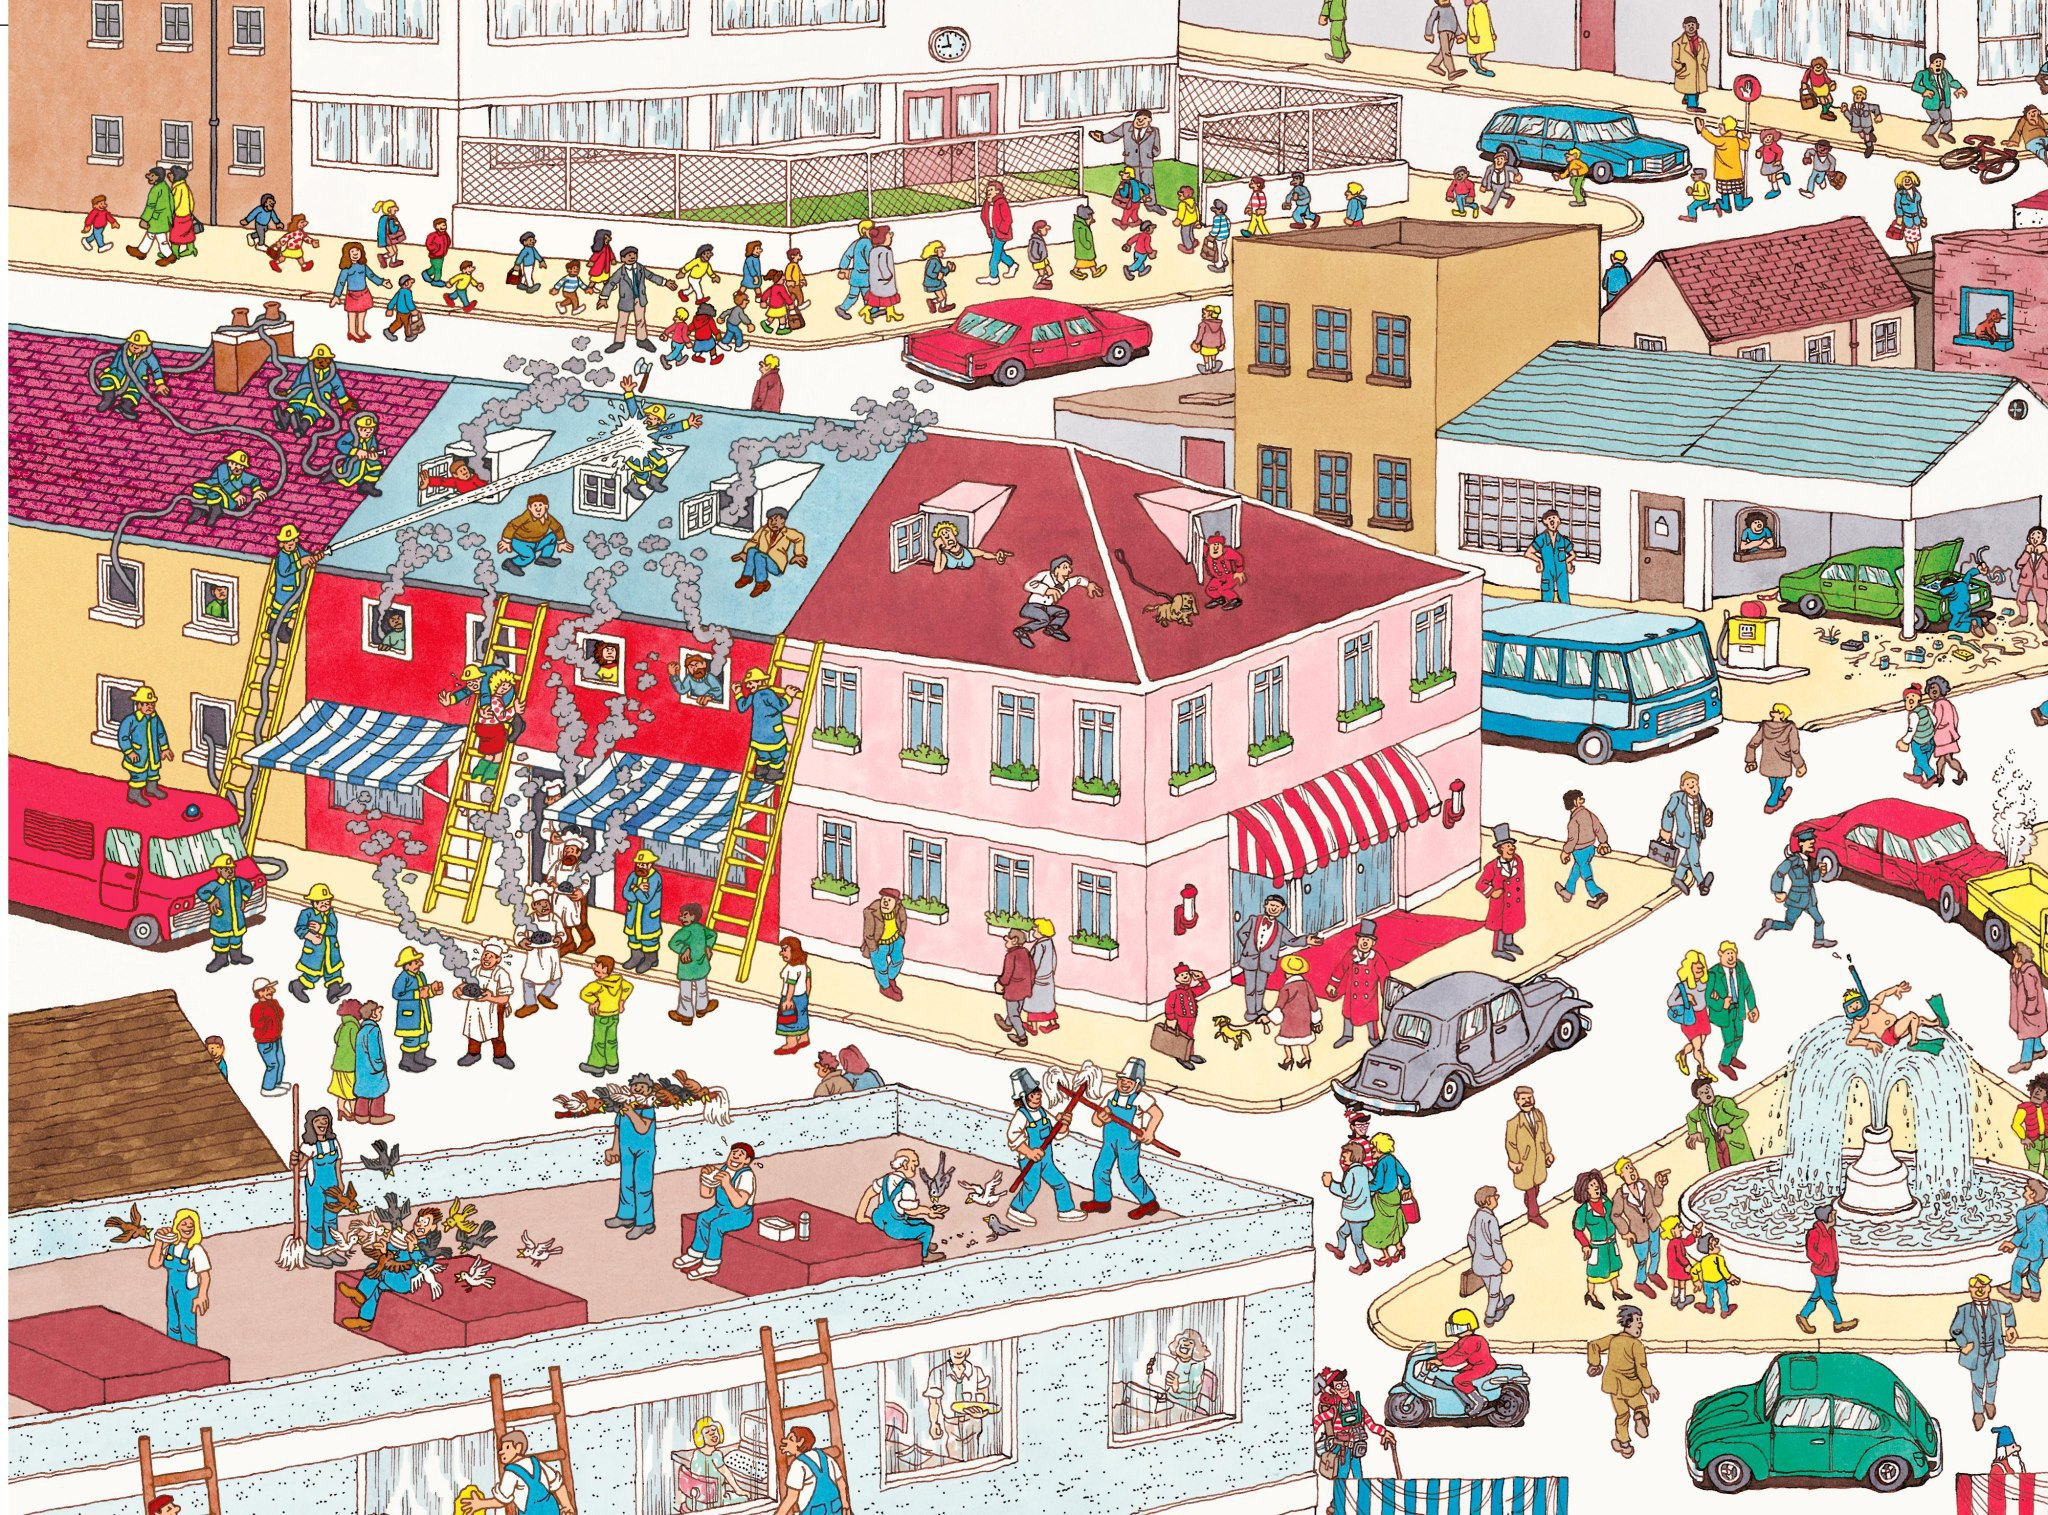
\includegraphics[width=0.9\textwidth]{wheres-wally}
            \end{figure}
        \end{center}

    \end{frame}
    
    \begin{frame}{SLAM} {Simultaneous Localization and Mapping}
      %More content goes here
      \vspace*{-1em}
      \begin{table}
        \begin{center}
          
          %\renewcommand{\arraystretch}{1.5}
          \begin{tabular}{m{0.4\textwidth} m{0.4\textwidth}} %{>{\centering\bfseries}m{1in} >{\centering}m{1in}}
            Navigation, & 
            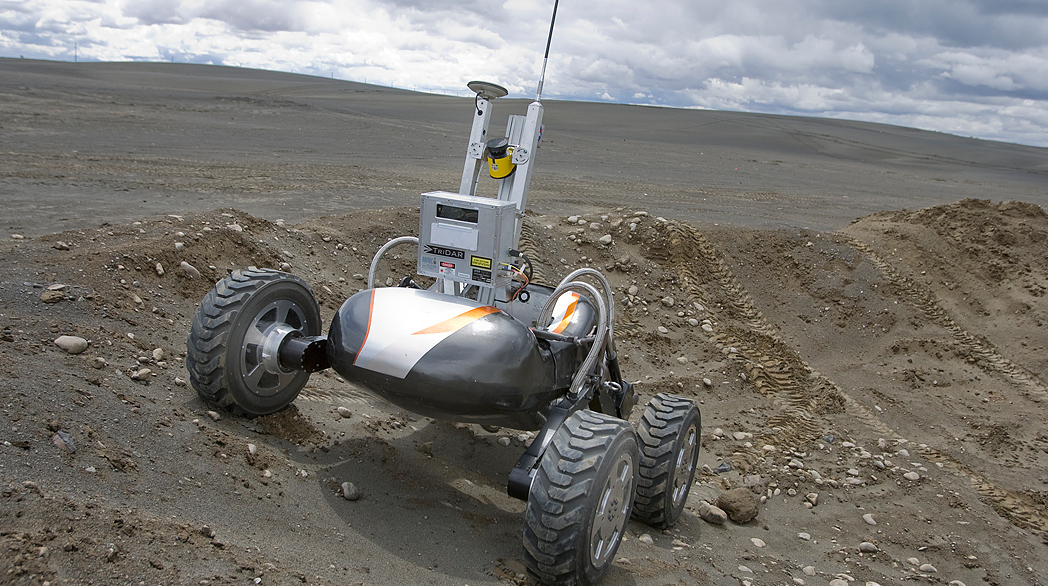
\includegraphics[width=0.4\textwidth]{navigation} 
            \\
            \begin{minipage}{0.4\textwidth}
              augmented\\reality,
            \end{minipage} & 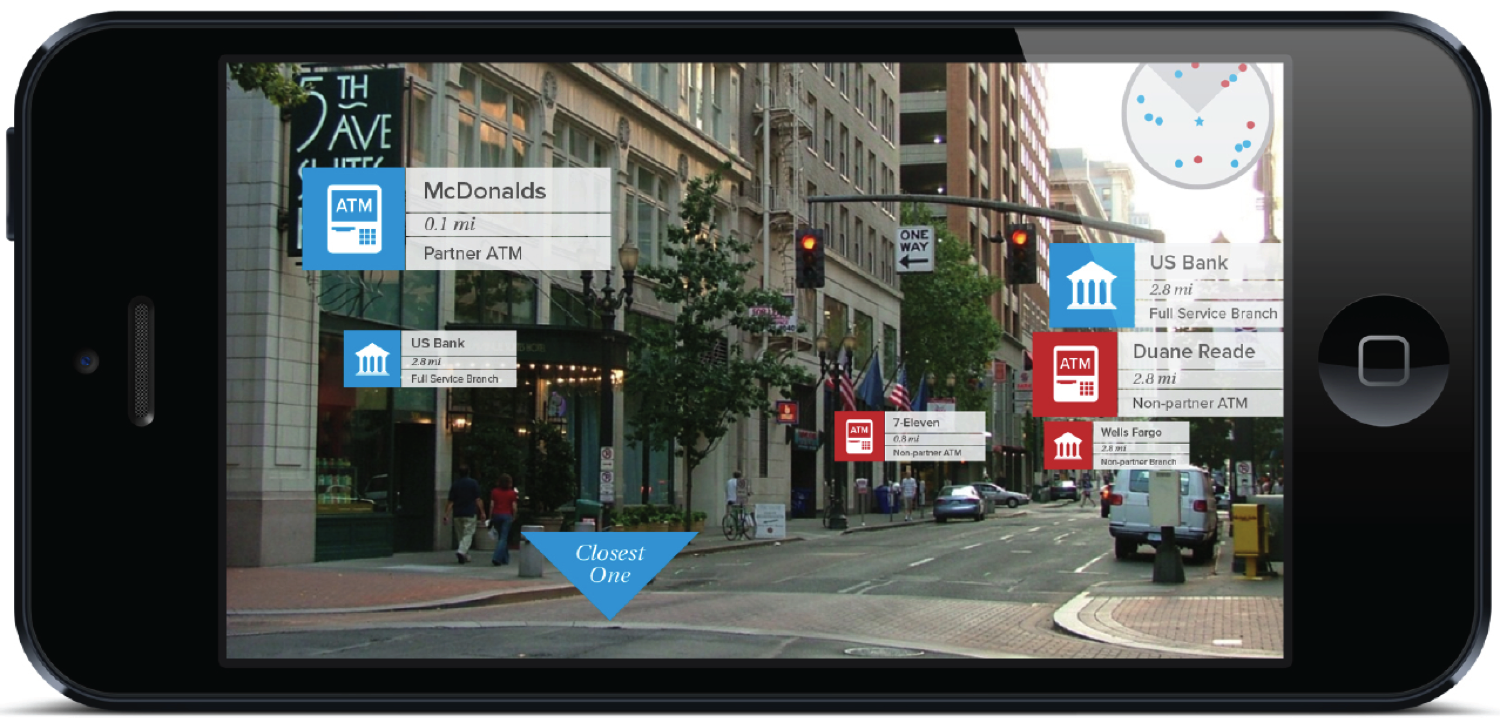
\includegraphics[width=0.4\textwidth]{augmented-reality-phone-for-blog}
            \\
            \begin{minipage}{0.4\textwidth}
              environment\\reconstruction
            \end{minipage} &
            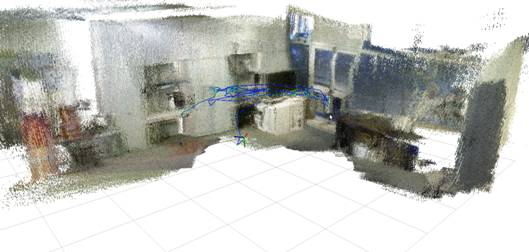
\includegraphics[width=0.4\textwidth]{EA-03}
          \end{tabular}
        \end{center}
      \end{table}
      
    \end{frame}
    
    \begin{frame}{SLAM} {Simultaneous Localization and Mapping}
      %More content goes here
      \vspace*{-3em}
      \begin{center}
        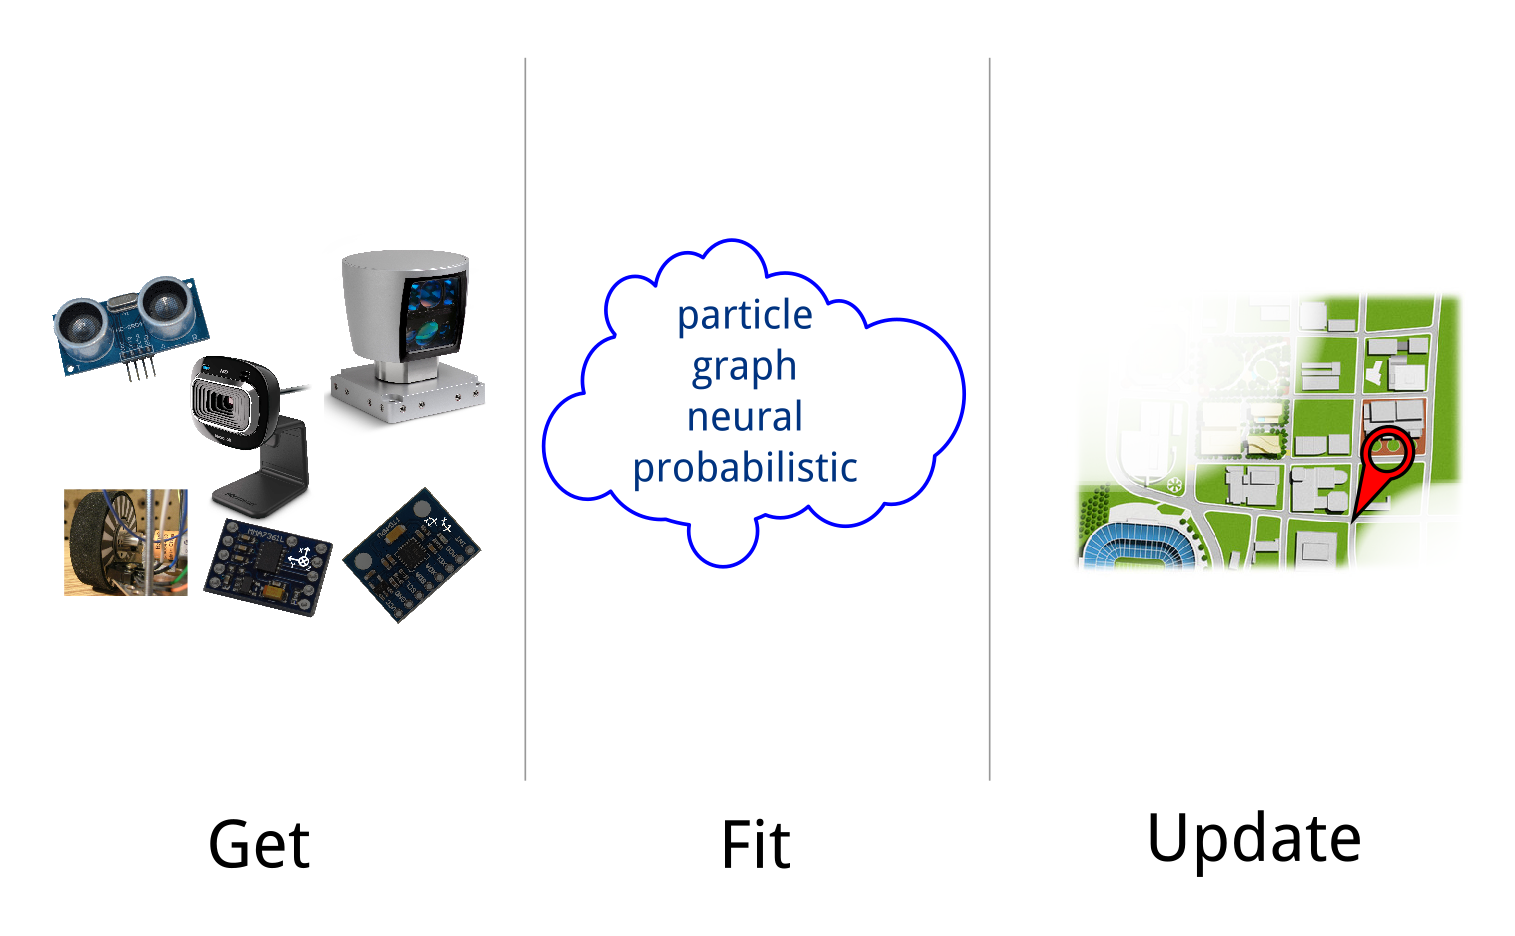
\includegraphics[width=\textwidth]{slam-alg}
      \end{center}
      
    \end{frame}
    
    \begin{frame}{Current senario} %{Spiking Neural Networks}
      %More content goes here
      \vspace*{-3em}        
      \begin{columns}[c] % the "c" option specifies center vertical alignment
        \column{.666\textwidth}
          \begin{itemize}
            \item Power hungry
            \item Exotic sensors
            \item Either indoor or outdoor
          \end{itemize}
        \column{.333\textwidth}
        \hspace*{-3em}
        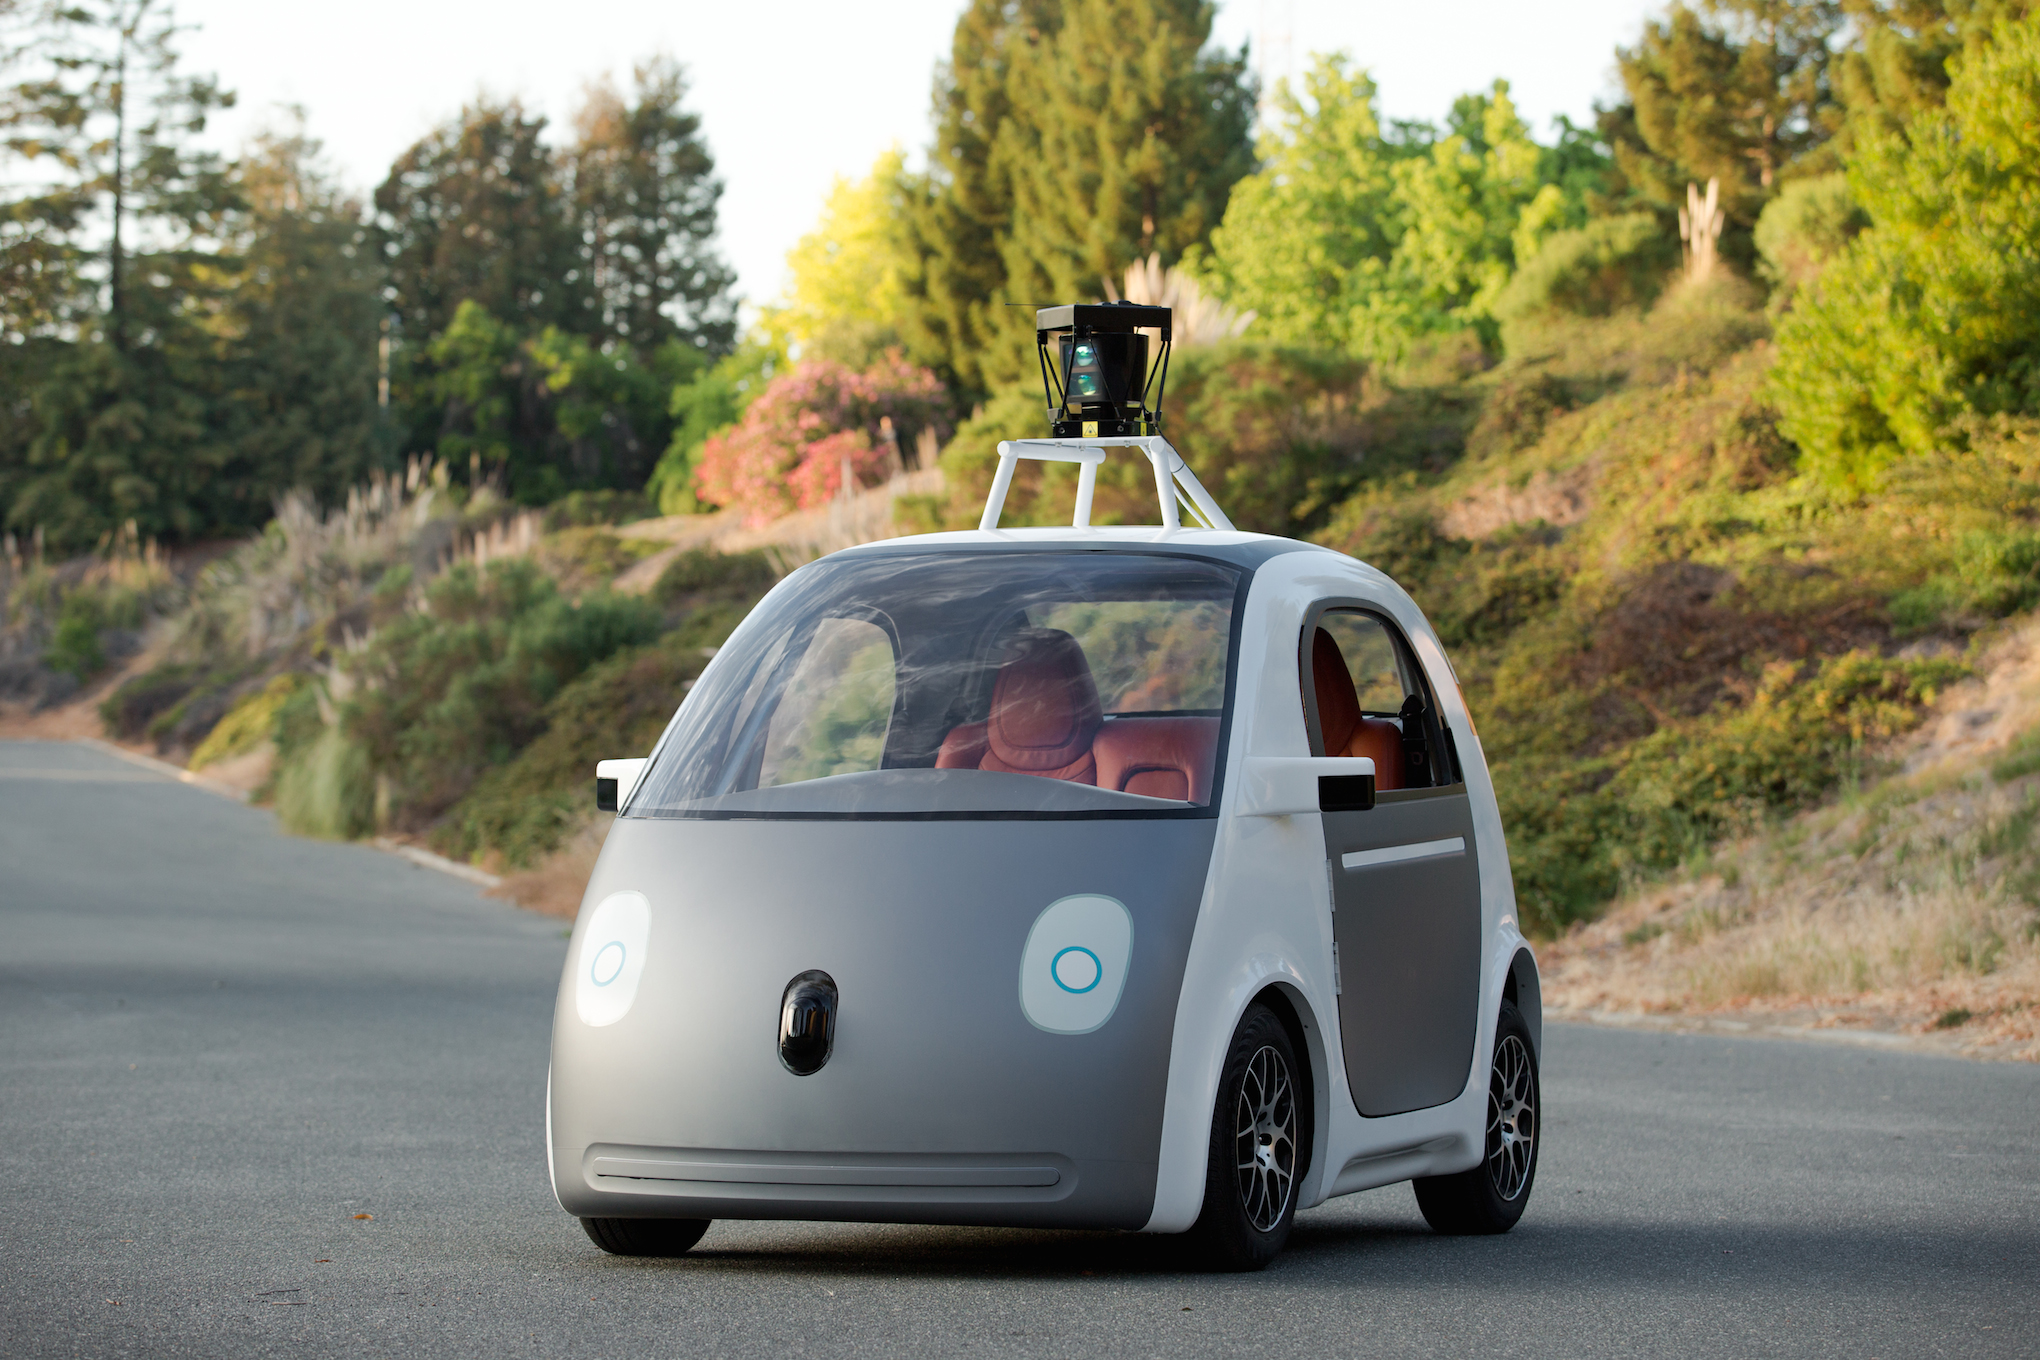
\includegraphics[width=1.5\textwidth]{Google_Self-Driving_Prototype__1_}\\[1em]
        \hspace*{-2em}
        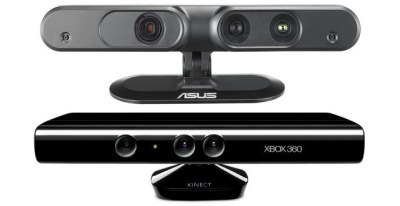
\includegraphics[width=1.2\textwidth]{kin}
      \end{columns}
    \end{frame}
        
    \begin{frame}{Neural Networks}{}
      %More content goes here
      \vspace*{-3em}        
      \begin{columns}
        \column{0.8\textwidth}
        \begin{itemize}
          \item Neural networks SLAM\cite{rat-slam}
          \item More efficient
          \item Neuromorphic hardware 
        \end{itemize}
        \column{0.35\textwidth}
        \hspace*{-1.em}
        \vspace*{-1em}
        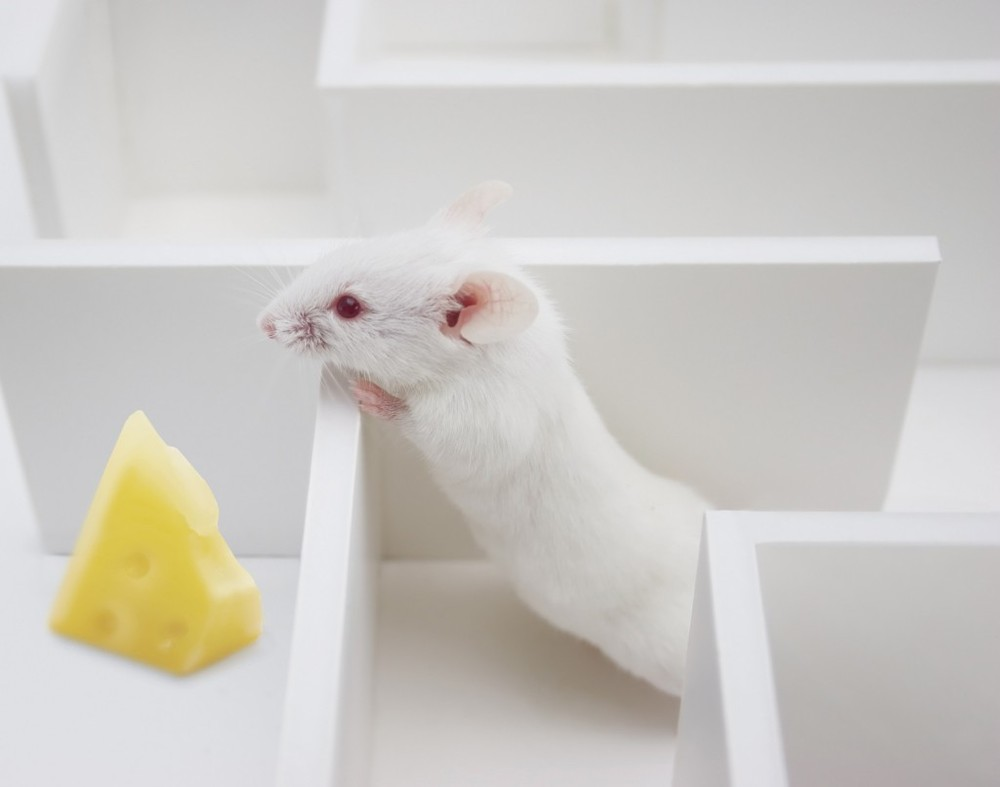
\includegraphics[trim={0 0 12cm 0}, clip, width=\textwidth]{rat-maze-cheese}
      \end{columns}
    \end{frame}

    \begin{frame}{Neural Networks}{}
      %More content goes here
      \vspace*{-3em}
      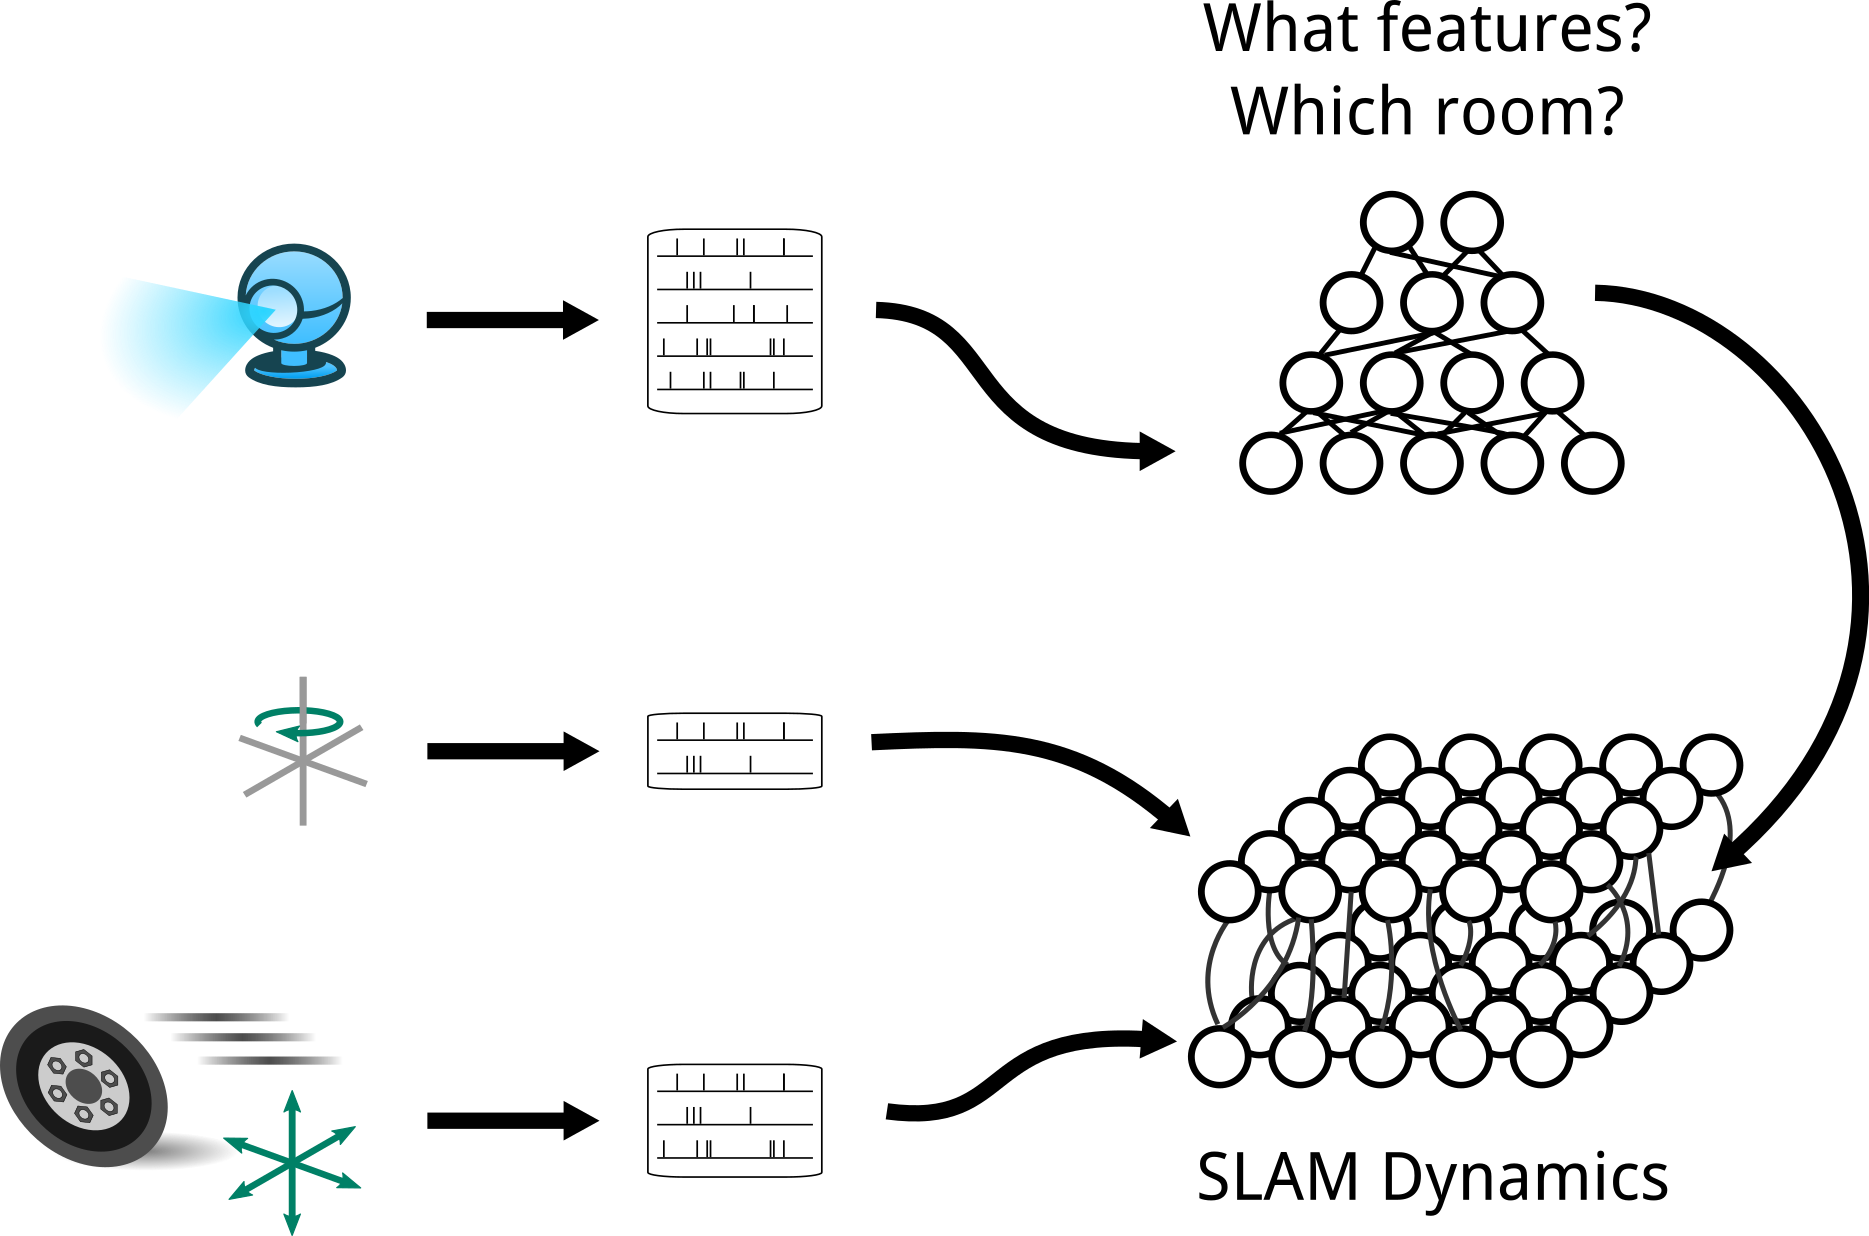
\includegraphics[width=\textwidth]{neuro-slam}
    \end{frame}

    \begin{frame}{Input System}
      %More content goes here
      \vspace*{-3em}
      \begin{figure}
        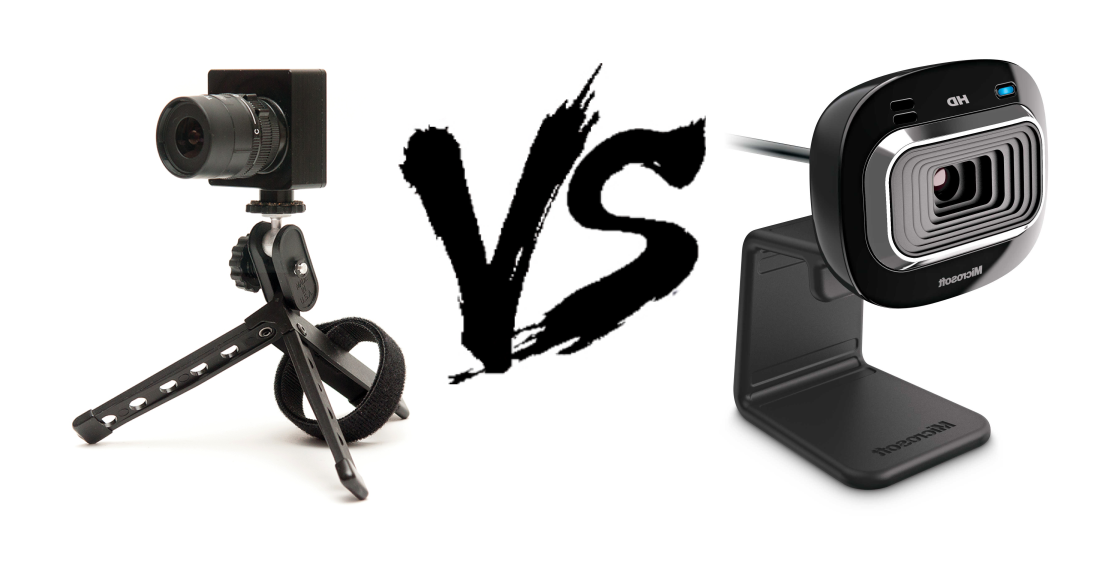
\includegraphics[width=\textwidth]{./dvs-vs-cam}
      \end{figure}
      \vspace*{-0.8em}
      \hspace*{0.05\textwidth}
      \begin{minipage}{0.9\textwidth}
        \centering \small How to get spiking visual input?
      \end{minipage}
    \end{frame}

    \begin{frame}{Input System}
      %More content goes here
        \vspace*{-4em}
        \begin{figure}
            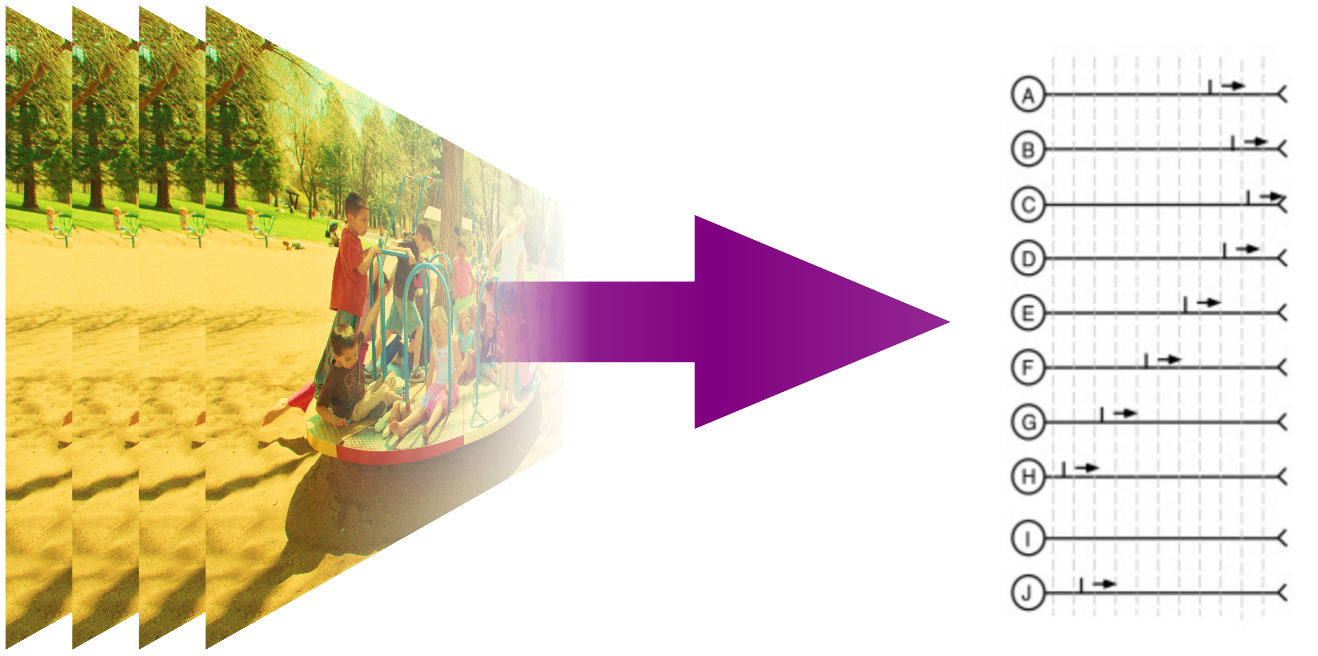
\includegraphics[scale=0.3]{./images-to-spikes}
        \end{figure}
        \vspace*{-0.4em}
        \hspace*{0.05\textwidth}
        \begin{minipage}{0.9\textwidth}
          \centering \small Convert images/video to spike trains
        \end{minipage}
    \end{frame}
    
    \begin{frame}{First encoder}
      \vspace*{-3em}
      \begin{itemize}
        \item Based on eye anatomy\cite{basab}
        \item Retains visual information
        \item 12 fps + correction algorithm
      \end{itemize}
      \vspace*{-1em}
      \begin{figure}
        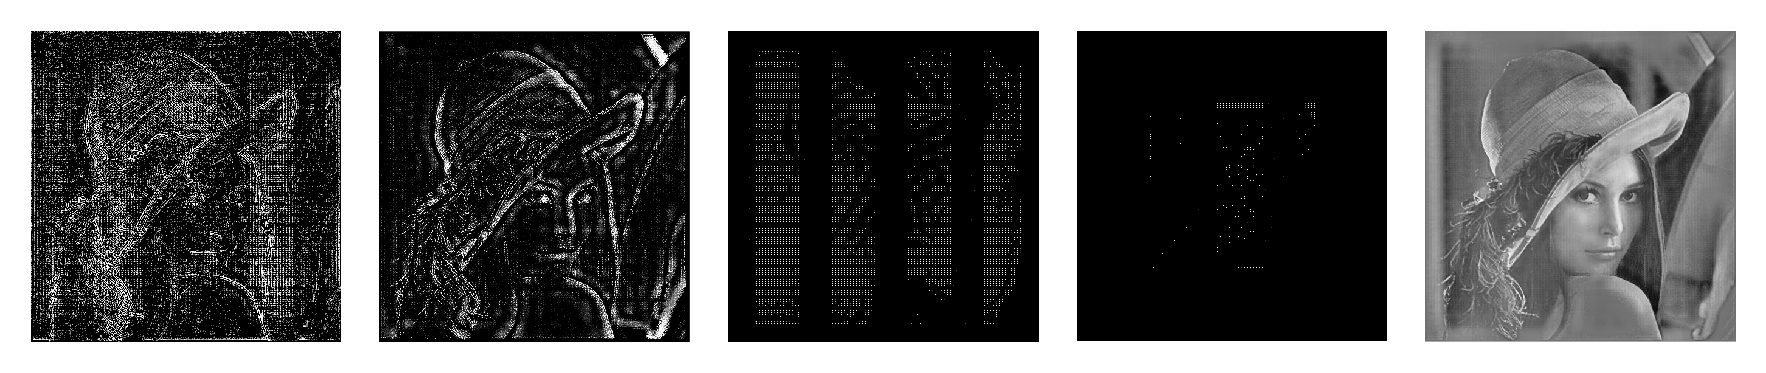
\includegraphics[width=\textwidth]{focal-imgs}
      \end{figure}
    \end{frame}

    \begin{frame}{Second encoder}
      \vspace*{-2em}
      \begin{itemize}
        \item Emulate Dynamic Vision Sensor 
        \item Sense changes in contrast
        \item Per-pixel adaptive threshold
      \end{itemize}
      \vspace*{-1em}
      \begin{figure}
        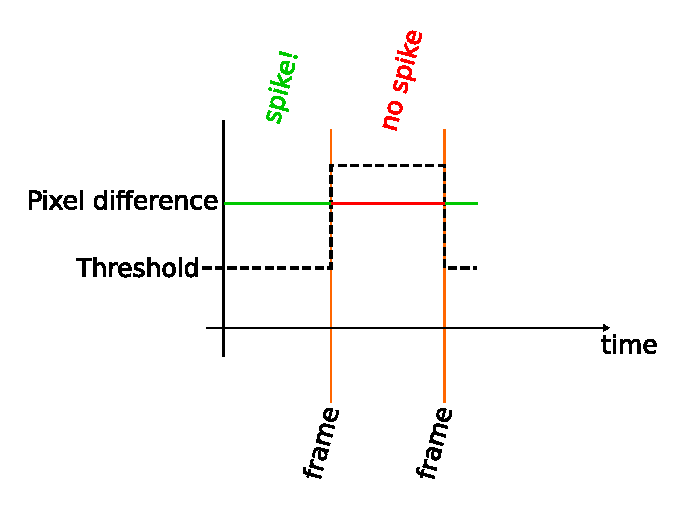
\includegraphics[width=0.4\textwidth]{DVSemu} 
        \hspace*{0.1em}
        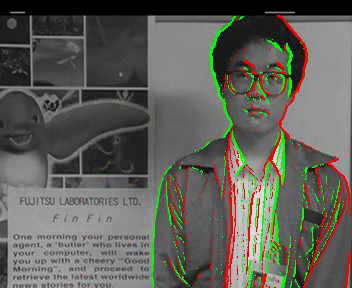
\includegraphics[width=0.4\textwidth]{dvs-emu-img}
      \end{figure}
    \end{frame}

    \begin{frame}{Final Words}
        %More content goes here
        \vspace*{-3em}
        \begin{itemize}
          \item[$\checkmark$] Familiarized with SpiNNaker \& reviewed state of the art
          \item[$\checkmark$] Video-to-spike encoder
          \item[$\checkmark$] Paper waiting to be reviewed in Frontiers
        \end{itemize}
    \end{frame}

    \begin{frame}{Final Words}
      %More content goes here
      \vspace*{-3em}
      \begin{itemize}
        \item[{\footnotesize [\textsc{to do}]}] On-line learning of spiking neural networks
        \item[{\footnotesize [\textsc{to do}]}] Object recognition and tracking with deep networks
        \item[{\footnotesize [\textsc{to do}]}] Spiking version of SLAM
      \end{itemize}
    \end{frame}

    \begin{frame}{The End}
      %More content goes here
      \begin{center}
          \vspace*{-3em}
          {\Large Thank You!}\\
          \vspace*{0.5em}
          Contact me:\\[1em]
          {\Large \textbf{pinedagg@cs.man.ac.uk}}\\
      \end{center}
    \end{frame}
    
    \begin{frame}{References}
      \vspace*{-3em}
      \printbibliography

    \end{frame}



\end{document}
